\documentclass{article}
\usepackage{graphicx}


\author{Martinez, Luis E\\
		Janicke, Marla}
\title{Ex 5.3}		
\begin{document}
\maketitle
	For this exercise we use the library of \textbf{Trixi.jl}, for the solution of DGSEM, where we use the Gauss-Lobatto-Legendre quadrature, all it's developed in the library
	\begin{figure}
		\centering
		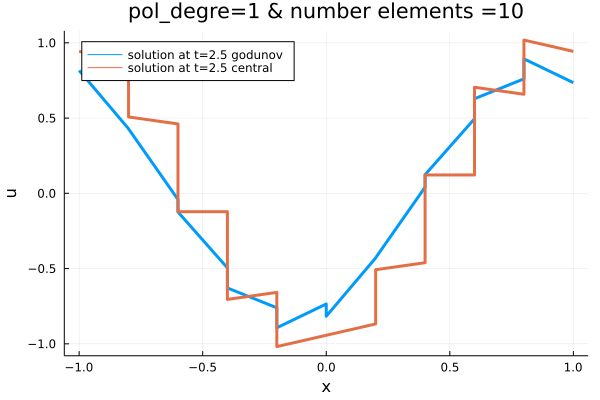
\includegraphics[width=6cm]{1,10}
		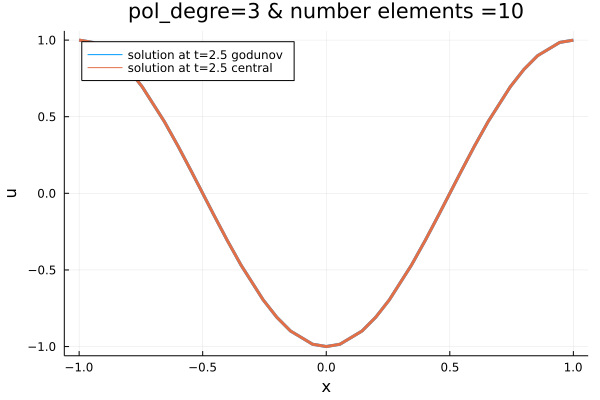
\includegraphics[width=6cm]{3,10}
		\caption{The same number of elements, we are changing the polynomial order and the fluxes}
	\end{figure}
	\begin{figure}
		\centering
		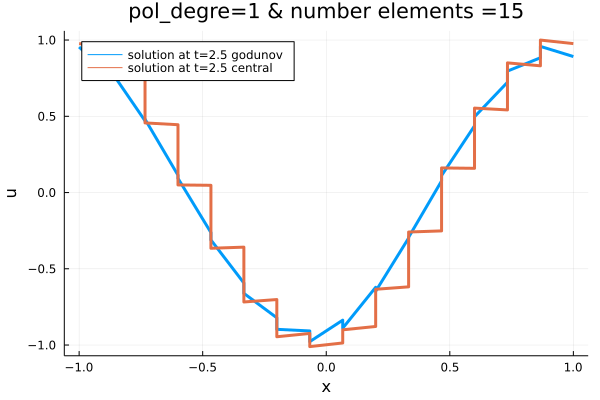
\includegraphics[width=6cm]{1,15}
		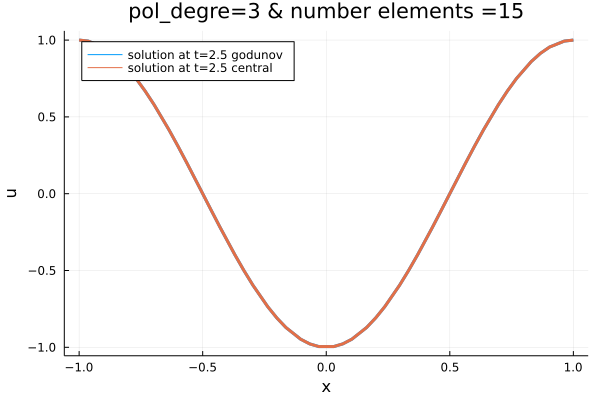
\includegraphics[width=6cm]{3,15}
		\caption{The same number of elements, we are changing the polynomial order and the fluxes}
	\end{figure}
	\begin{figure}
		\centering
		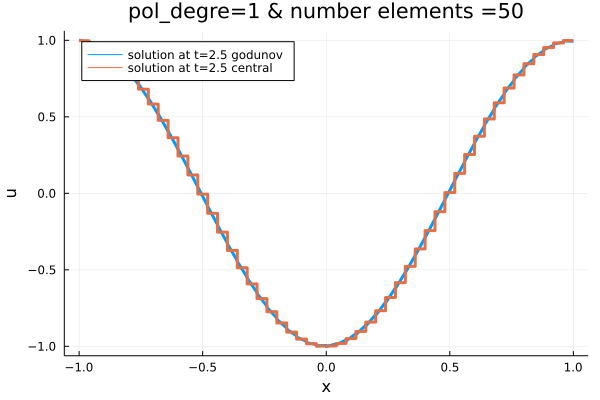
\includegraphics[width=6cm]{1,50}
		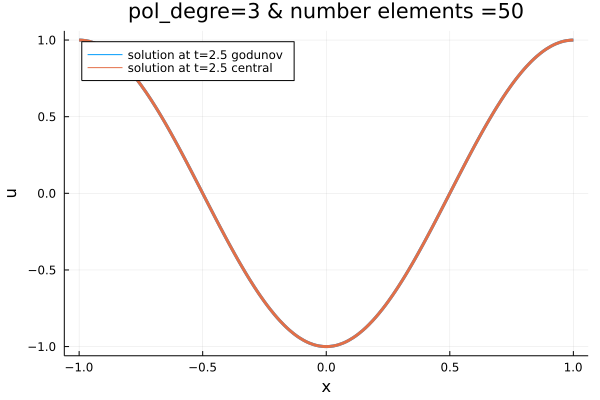
\includegraphics[width=6cm]{3,50}
		\caption{The same number of elements, we are changing the polynomial order and the fluxes}
	\end{figure}
	As we can see in these graphics, for polynomial degree$=3$ the behavior it's almost the same, maybe there is a difference but we cannot distinguish only looking at the graph, for polynomial degree$=1$, the  central flux, is worst than the godunov flux, we discuss what could be the origin of this, but we couldn't get a satisfactory answer, It is left as an exercise for the reader.\end{document}
